\chapter{Related Work}
\label{chapter:related-work}


In this chapter, we discuss earlier relevant work in the area of improving the
performance of Web services in \gls{dil} environments. Improving Web services is
important for both civil and military users as increasing the performance means
that applications can become faster and more reliable.

In the following sections, we identify studies and recommendations that are
applicable to this thesis. We get started by looking into the work of the NATO
research groups IST-090 and "SOA Recommendations for Disadvantaged Grids in the
Tactical Domain" (IST-118). IST-118 is an ongoing follow-on to the work of
IST-090, with the goal of creating a recommendation for a tactical profile for
using SOA in disadvantaged grids. Next, based on these recommendations, we
investigate work done in the area of alternative transport protocols and
existing proxy implementations.  Finally, we summarize the findings that are
applicable with regards to the scope and premises of this thesis.

\section{Making SOA Applicable at the Tactical Level}

IST-118 has published a paper\cite{ist-118} where they summarized the findings
of IST-090. Although the paper only looked into W3C Web services, many of their
recommendations are also applicable to RESTful Web services. They identified
three key issues that need to be addressed in order to adopt Web services in
tactical networks:

\label{section:DIL-problems}

\subsubsection{1. End-to-end Connections}

Web services mostly use transport protocols that depend on a direct, end-to-end
connection between a client and the service. Attempting to establish and
maintaining a connection in a DIL environment can lead to increased communication
overhead and the possible complete breakdown of communication. Most Web services use
TCP as their transport protocol, which relies on an uninterrupted connection.
In DIL environments with high error rates and high latencies,
the congestion control of TCP can cause sub-optimal utilization of the network
as previously discussed in \cref{section:tcp-problems}. Similar, HTTP, which is
the application layer protocol most often used together with TCP, struggles in
such environments. HTTP is a synchronous protocol, which means that the HTTP
connection is kept open until a response is received. Long response times could cause
timeouts. IST-090 points out the possible solution of replacing HTTP and TCP with
other, more suitable protocols.

The IST-90 report mentions two approaches to replace HTTP/TCP. The clients and
services themselves can be modified to support other protocols, or proxies
which support alternative protocols can be used \cite{ist-090}. Moreover, they
pointed out that if using a proxy approach, standards compliance can be
retained.


\subsubsection{2. Network Heterogeneity}

Another issue is when heterogeneous networks are interconnected. Different
performance in networks may lead to buildup of data in buffers, risking loss of
information. A proposed solution to this is to have store-and-forward support
which can support that messages are not dropped, but rather stored and forwarded when
possible.


\subsubsection{3. Web Service Overhead}

W3C Web services are associated with a considerable amount of overhead. Web
Service technology is based on SOAP, which uses XML-based messages. It is a
textual data format and produces much larger messages than binary formats.
Optimization approaches should seek to reduce the network traffic generated by
Web services by using techniques as compression to reduce the size of messages.
Another approach is to reduce the number of messages being sent, which was
looked into in IST-090 \cite{ist-090}. In their work they investigated three
different ways to do this:

\begin{enumerate}
    \item Employing caching near the client in order to reuse older messages.
    \item Using the publish-subscribe paradigm, which allows clients to subscribe to
    information instead of requesting it. This allows the same message to be sent
    to multiple clients.
    \item Employing content filtering which filters out unnecessary data.
\end{enumerate}

The scope of this thesis is to optimize for request-response type of clients and
Web services. Furthermore, since we are investigating general-purpose
optimization techniques without knowledge of the payload, some of these
recommendations does not quite apply to us. However, to reduce Web service
overhead we can apply the well-known technique of compression.

\subsubsection{Compression}

Data compression is the technique of encoding information using fewer bits than
the original representation. In a network with limited data rate, the reduction
would significantly reduce time used to send the data. The reduction of data is
often expressed in the term \textit{compression rate}, which expresses the ratio
between the uncompressed size and compressed size of the payload.  Moreover,
there exist two types of compression, \textit{lossy} and \textit{lossless
compression}. Lossy compression is used to compress data such as images and
movies where the consequence of losing some of the data is not critical.
Lossless compression utilizes repeating patterns in the data in order to
represents the same data in a more efficient way.

\gls{xml} is the data format used by W3C Web services and has a significant
overhead. A previous study evaluated different lossless compressions techniques
for exchanging XML documents using W3C Web services \cite{johnsen-compression}.
They evaluated both XML-specific and general purpose (payload agnostic)
compression techniques. There exist a great number of different compression
techniques, so the authors focused on a few they saw as promising for use in
tactical communication networks. The first one, \gls{efx}, encodes XML documents
in a binary instead of textual format. The two other were the XML-specific XMLPPM
and general-purpose compression tool GZIP.

In their evaluation, they saw that for all techniques, larger XML documents
achieved a higher compression ratio than smaller documents. As the average, EFX
applied with a built in proprietary ZIP enabled had the highest compression
ratio followed by GZIP. However, they concluded that all evaluated techniques
provided a significant reduction of payload size, so the specific technique was
of less importance.

\section{TACTICS TSI Architecture}

Another ongoing effort to overcome issues using standard Web services in
tactical networks are the TACTICS project supported by the \gls{eda}
\cite{tactics-diefenbach}. The goal of the project is to propose a reference
architecture for a \gls{tsi} suited for establishing a tactical \gls{soa} of
defence-related information systems. The architecture features a service
middleware meant to run on devices with different capabilities. The purpose of
the middleware is to receive standard Web service invocations or responses and
ensure that they complete. The middleware can forward IP packets between
different radio networks and store and forward messages.

\section{Previous Evaluations of Alternative Protocols}

A previous study has investigated potential gains from replacing HTTP/TCP with
alternative protocols \cite{evaluation-transport-protocols-web-services}.
\Citeauthor{evaluation-transport-protocols-web-services} looked into TCP, UDP,
SCTP and AMQP for conveying Web services traffic under typical military
networking conditions. The researchers found that \gls{sctp} had the highest
success rate in military tactical communication. However, on links with the
lowest data rate, the protocol tended to generate more overhead than TCP. They
pointed out that this was due to SCTP having a more complex connection handshake
procedure and in addition using heartbeat packets.

Another study has compared the performance of MQTT and \gls{coap} in terms of
end-to-end delay and network usage \cite{thangavel-mqtt-coap}.
\Citeauthor{thangavel-mqtt-coap} performed experiments in different emulated
networks with varying message sizes and loss rates. They saw that both MQTT and
CoAP were successfully able to handle packet losses of up to 25 \%. With lower
loss rates, messages sent with MQTT had the lowest delay, but as the loss rate
increased CoAP had lower delay. They identified the reason for this being that
the TCP transmission of MQTT had a larger overhead than CoAP's UDP transmission.
In their experiments with small message sizes and for all tested loss rates, did
CoAP have less network overhead than MQTT. However, as the message size grew was
the opposite true.

Another comparison of CoAP and MQTT was done in a study using the protocols for
sensing applications running on a smartphone \cite{caro-mqtt-coap}. This study
also confirmed CoAP as having lower network usage and a lower RTT. However, the
study pointed out that MQTT has more advanded \gls{qos} services, since it can
guarantee exactly once delivery of messages. Since CoAP does not have this
feature, applications which require this feature should consider using MQTT.

CoAP has also been compared against HTTP in a work done by
\citeauthor{walter-coap-http}, where they performed an evaluation with regards
of response time and energy consumption by a sensor node
\cite{walter-coap-http}. They found that using CoAP consumed significantly lower
energy than using HTTP, and that CoAP also had  a lower response time.

\section{Proxy Optimization}

One of the recommendations of IST-090 was the usage of proxies. This
recommendation has been picked-up by other research groups and a set of proxies
for optimizing Web services in DIL networks already exist. However, many of them
do not fulfill all the requirements we have for our proxy. Some of them do
only support SOAP Web services and others are unusable due to security reasons.
This section lists and discusses previous implementations of such proxies.

\subsection{Types of Proxies}

A proxy is a node deployed somewhere in a network, which through network traffic
can pass. Proxies has many use cases such caching, firewalling and security. In
order to adopt Web services into tactical networks we mainly talk about two
types of proxies. Edge proxies act as gateways between different networks as
illustrated in \cref{figure:edge} and can perform adaptations on network traffic
passing between.

\begin{figure}[h]
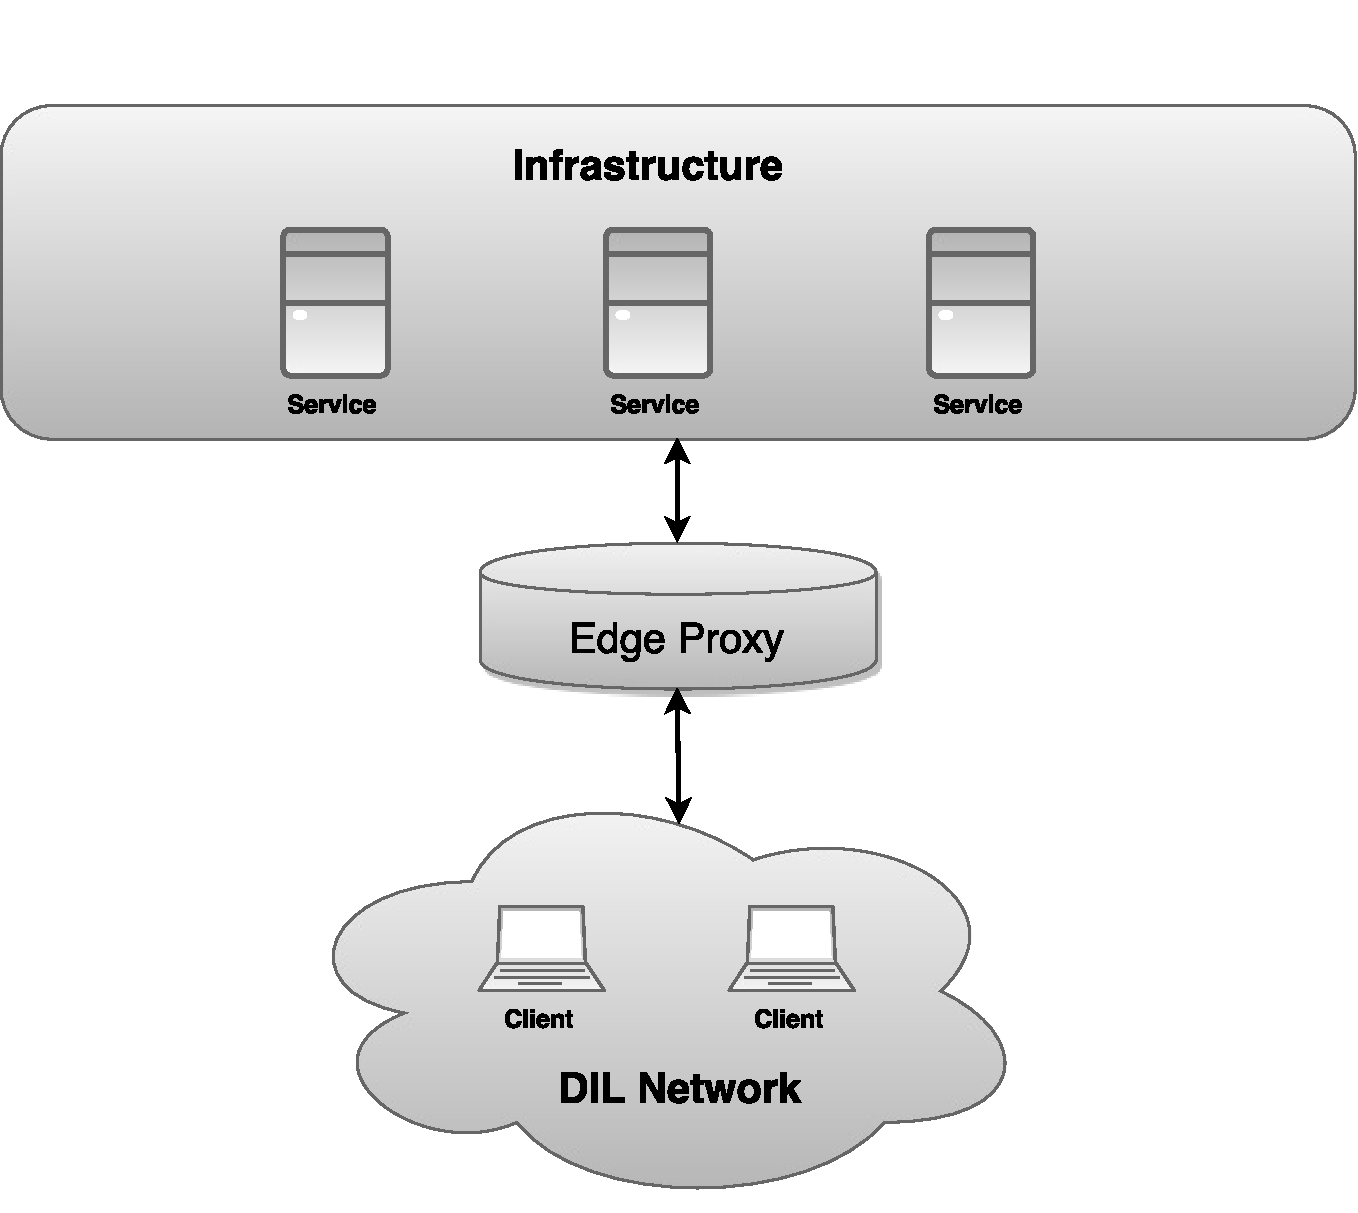
\includegraphics[scale=0.35]{images/edge_proxy.pdf}
\caption{Edge proxy}
\label{figure:edge}
\end{figure}

Another type is point-to-point inside a network as illustrated in
\cref{proxy-point}, and involves using a proxy-pair to facilitate communication
between two or more applications.

\begin{figure}[h]
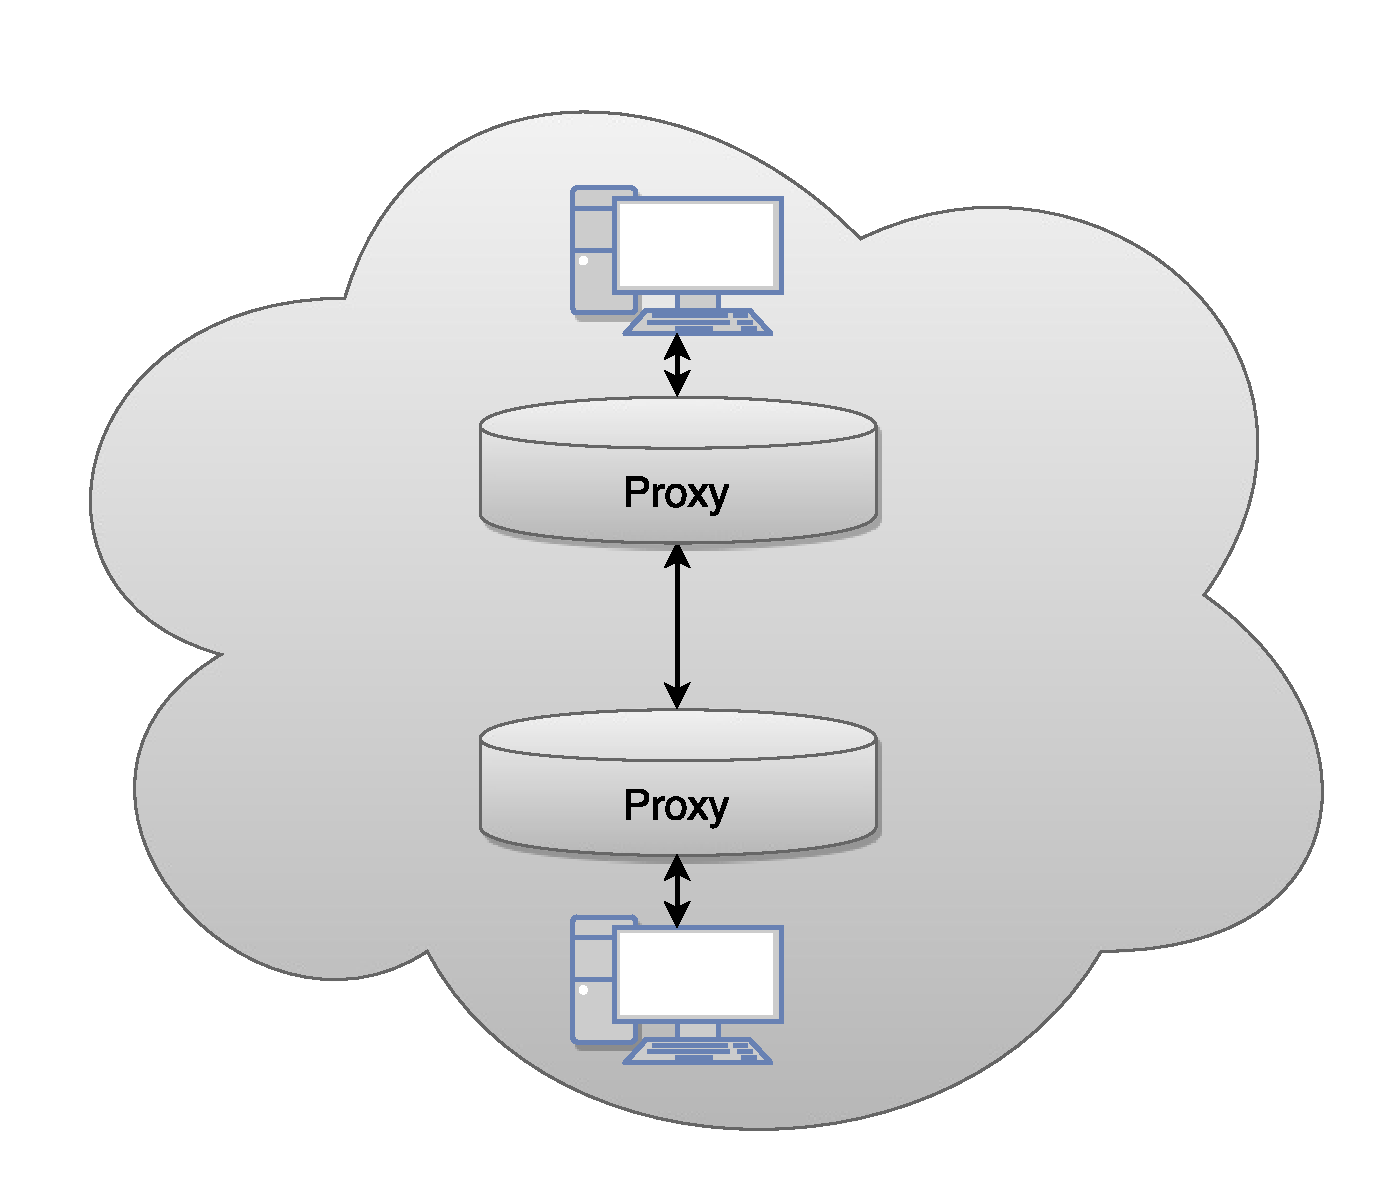
\includegraphics[scale=0.35]{images/proxy_point.pdf}
\caption{Point-to-point proxy}
\label{figure:proxy-point}
\end{figure}

\subsection{\glsentrylong{dsproxy}}

The \gls{dsproxy} is a proxy solution developed by \gls{ffi}
\cite{dsproxy-ffi}\cite{ieee-dsproxy}. Its goal was to enable the usage of
unmodified standard W3C Web services (SOAP over HTTP/TCP) in DIL environments.
The concept was to route all SOAP messages through the proxy. When the proxy
received a message, it was stored locally before it was forwarded. If the
forwarding failed for some reason, it could retry the request until it
eventually succeeded. This ability, called \textit{store-and-forward}, was one
of the fundamental core functionalities of \gls{dsproxy}. When a request
eventually succeeded, the response was returned to the client on the original
TCP connection initiated by the client. By doing this, Web service invocations
were made possible over unreliable networks by hiding any network disruptions
from the client.

\begin{figure}[h]
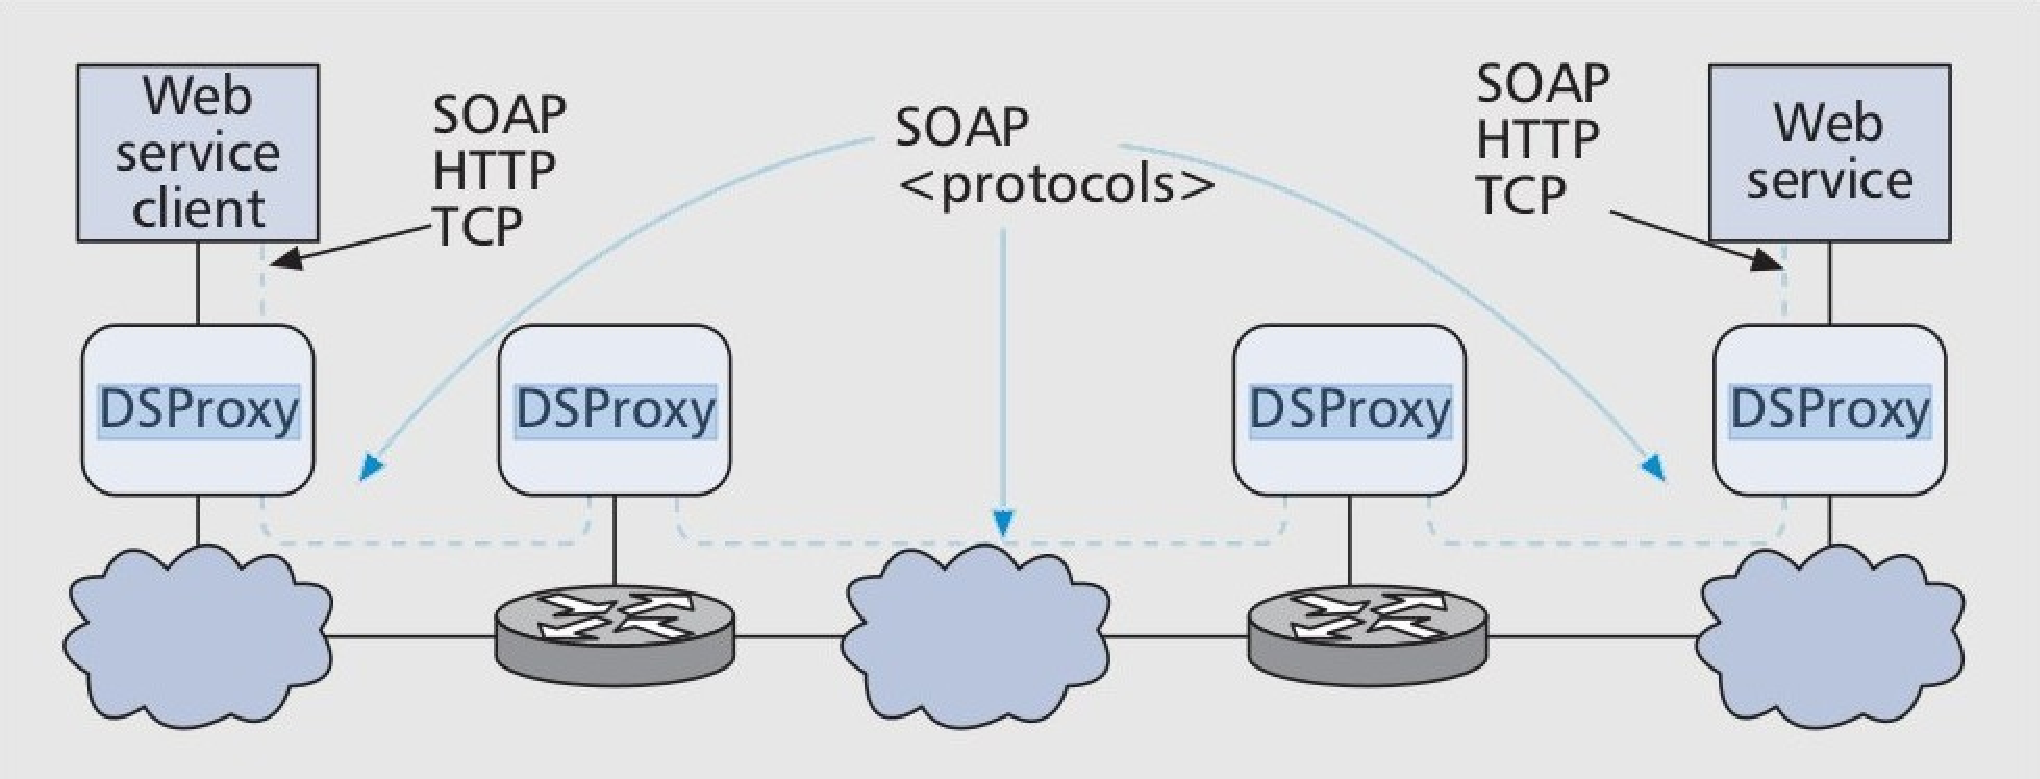
\includegraphics[scale=0.35]{images/dsproxy.pdf}
\caption{DSProxy overlay network (from \cite{ieee-dsproxy} )}
\label{figure:dsproxy}
\end{figure}

Another core functionality of DSProxy was mechanisms for organizing an overlay
network consisting of multiple proxy instances as seen in \cref{figure:dsproxy}.
This enabled the ability to traverse multiple and heterogeneous networks, but
also added a lot of complexity to the proxy application. Apart from the
mentioned core functionalities, DSProxy supported a set of pluggable
functionalities such as GZIP compression and caching.

After performing experiments using the DSProxy, the researchers identified the
store-and-forward ability as very important in unreliable networks in order to
avoid having to re-establish end-to-end connections each time the network
connections was lost \cite{dsproxy-ffi}. One of the downsides with DSProxy was
that it only supported W3C Web services. Moreover, it became very complex due to
its mechanisms for building overlay networks and supporting different
configurations and plugins.

\subsection{NetProxy}
%https://www.researchgate.net/profile/Niranjan_Suri/publications

NetProxy is another network proxy solution aiming at enabling SOA applications
for use in DIL environments \cite{suri-netproxy}. The proxy is a component of
the \gls{acm}, a set of components that satisfy many of the communications
requirements found in challenged networks. The work is being carried out by
researchers at the Florida Institute for Human \& Machine Cognition.

Like DSPRoxy, NetProxy is a transparent proxy providing integration between SOA
systems without requiring modification of applications themselves. It works by
first intercepting all network traffic from the applications and then do an
analysis of it. Together with information about the network, NetProxy then
decides which appropriate action to take. It can be configured to support
protocol remapping by using other protocols than HTTP/TCP. Integrated with
NetProxy is the message-oriented transport protocol \gls{mockets}, which is
designed to replace \gls{tcp} and \gls{udp} and is targeted for DIL networks
\cite{suri-netproxy}. Mockets replaces the congestion control and reliable
transmission algorithms of TCP with other alternate implementations designed for
DIL networks. It is configurable for different types of networks and offers
various \gls{qos} levels.

Performance testing of W3C Web services showed that using NetProxy with Mockets as
the transport protocol yielded a significant increase in the performance
compared to plain TCP \cite{suri-netproxy}. The researcher attributed this to
several factors:

\begin{itemize}

    \item Mockets handles packet loss much better than TCP since TCP attributes
    packet loss to congestion and triggers its congestion control.

    \item NetProxy multiplexes all network traffic directed to a single node
    onto the same connection and holds it open instead of closing it after a
    finishing request. This allows reusing the connections across consecutive
    requests, also from other applications.

    \item Less overhead due to NetProxy buffers data until it fills an
    entire packet before sending it over the network.

    \item Enabling compression gave a very high gain in the measured network
    throughput partly due to the messages subject for compression was XML
    documents, which have a relatively high compression rate.

\end{itemize}

\subsection{AFRO}

\gls{afro} is an edge proxy which offers different levels of \gls{qos} to Web
services through performance monitoring and usage of the context-aware service
provision paradigm \cite{ist-090}. It performs so called adaption actions, which
modifies the SOAP XML messages by changing their encoding to more efficient data
representation. \gls{afro} also removes information that is acceptable to be
removed by the service requester.

However, since the proxy modifies the data being sent, the digital signature of
the data is also changed. In applications where we want to be sure that no one
has tampered with the data before arriving, digital signatures are often used.
Consequently, this solution would not work for such applications.


\section{Tuning Application Server Parameters}

 Another approach to improve the performance of Web services is to configure
 the way they are deployed. Web services can be deployed in applications
 servers, which is a software framework that provides an environment where the
 Web services can run. When setting up an application server, several parameters
 which can affect the performance of running applications can be
 configured. Wrong or bad configuration may cause inaccurate timeouts and
 congestion in the network. In a paper written by researchers at \gls{ntnu} and
 FFI \cite{johnsen-recommendations}, they
 investigated how tuning the server parameters of the application server
 Glassfish affected the performance of both \gls{rest} and SOAP Web services.
 They identified a number of key HTTP and TCP tuning parameters:

\paragraph{HTTP Timeout} Controls how long a HTTP connection can be deemed as
idle and kept in the "keep-alive" state. Having a too low timeout on networks
with low data rate, can potentially flood the network with packets that have
timed out. Consideration should therefore be taken when setting this
parameter for mobile tactical networks.

\paragraph{HTTP Compression} Enables HTTP/1.1 GZIP compression.

\paragraph{HTTP Chunking} Allows the server to send data in dynamic chunks.

\paragraph{HTTP Header and Send Buffer Sizes} Vary the size of the buffers
that hold the request and send the data.

\paragraph{TCP Idle Key Timeout} Sets the time before an idle TCP channel
closes.

\paragraph{TCP Read and Write Timeouts} Set the timeout for TCP read and write
operations, respectively.

\paragraph{TCP Selector Poll Timeout} Sets the time a \gls{nio} selector will
block waiting for user requests.

\paragraph{TCP Buffer Size} Sets the size of the buffer that holds input streams
created by the network listener.

\paragraph{TCP Batching/TCP NO\_DELAY} Batches together small TCP packets into
larger packets.

\paragraph{MTU Size} The maximum transmission unit size regulates the largest
data unit that can be passed onwards. In tactical military communication the MTU
size can be very low (down to 128 bytes).

\paragraph{}
After running their experiments they concluded that few of the parameters
actually had any significant impact on the performance of the Web Service.
However, they identified HTTP Chunking configuration as having the most impact
on the performance. It significantly improved the performance in different types
of networks and for both SOAP and RESTful Web services.


\section{Summary}

In this chapter, we looked into efforts previously undertaken in order to improve
the performance of Web services in networks with the DIL characteristics. The
most important findings are summarized in \cref{table:related-work-summary}. We
first looked into the work of the research groups IST-090 and IST-118, and saw
how they identified end-to-end connections and Web service overhead as major
issues for enabling Web services in DIL environments. To overcome these issues,
they recommended the usage of proxies and several techniques for reducing the
overhead. We identified GZIP and EFX with zipping as important compression
techniques to reduce the size of Web service messages sent over a network. Next,
we looked into previously developed proxies for DIL networks. Although many of
them showed promising results, some of their properties did not fulfill the
premises for this thesis. They were either limited to SOAP-based Web services or
are inadequate to be used due to security reasons. However, we identified some
of their techniques that we carry on in the proxy developed in this thesis.

Finally, we investigated previous attempts with the usage of alternative
transport protocols, before we looked into previous efforts in the area of
tuning application server parameters. Based on recommendations and studies of
previous work, we are in the next chapter deriving a set of requirements for our
proxy.

%%%%%%%% TABLE OPTIMALIZATION OVERVIEW %%%%%%%%%%%%%
\begin{table}[h]
\begin{tabularx}{\textwidth}{| X | X |}
\hline
  \textbf{DIL Issue} & \textbf{Findings} \\ \hline

  Reduce Web service overhead  & Use compression techniques like GZIP or EFX
  with zip.\\ \hline

  End-to-end connection dependency & Use proxies. \\ \hline

  Alternate transport protocols & Summary here. \\ \hline
\end{tabularx}
\caption{Related work summary.}
\label{table:related-work-summary}
\end{table}
